Artificial intelligence, also referred to as statistical learning or machine learning, has become the buzz word of modern computing. While the inner workings of most machine learning techniques are overlooked by many disciplines, the end results speak for themselves. Machine learning techniques allow for adaptable models to be applied to a variety of problems. Traditional statistical methods require a deep understanding of the mathematics behind the algorithm, which can lead to an increase in the time to obtain a result. Machine learning algorithms do not require as deep of an understanding, but the reduced level of understanding required comes at the cost of  interpretability. Parameters within models like Least Squares Regression can be interpreted directly, allowing for researchers to obtain a deeper understanding of what the model achieves. 

Neural networks, sometimes called multilayer perceptrons, will be the focus of this paper. These particular models involve an input layer, a hidden state, and an output layer. A visualization of a nueral network is shown in Figure \ref{fig:NueralNetwork}.

\begin{figure}[ht]
    \centering
    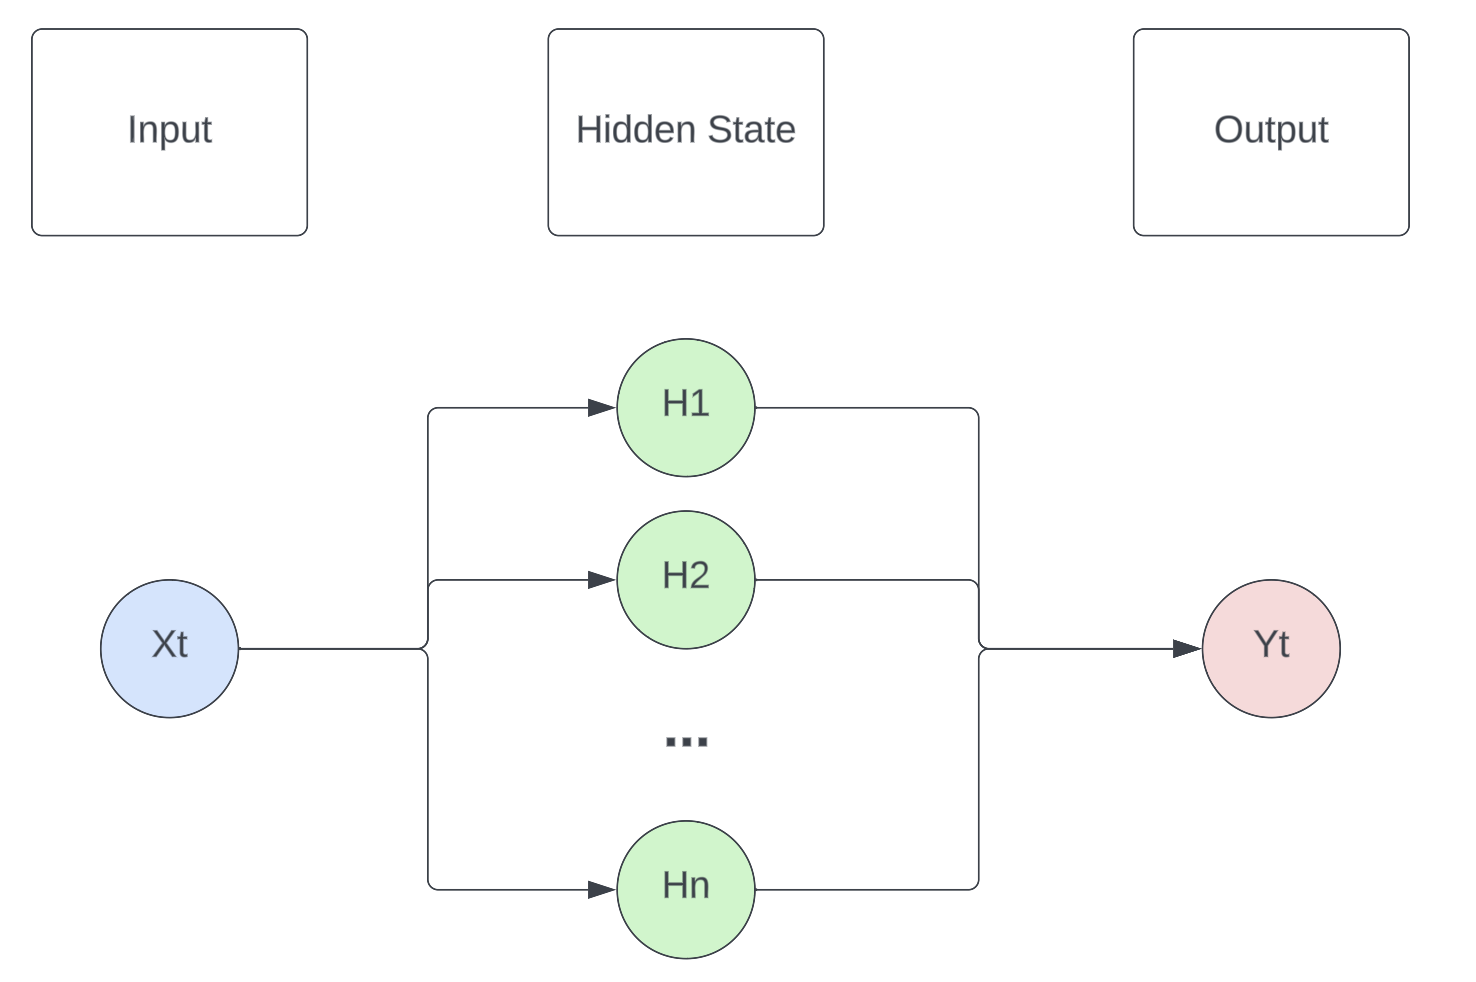
\includegraphics[width=0.6\linewidth]{"Figures/Traditional_NN.png"}
    \caption{A flowchart depicting a single-layer Neural Network. The input layer (blue) contains a single node, indicating a single value would be taken as an input. The hidden state (green) contains a single layer of \textit{n} nodes. The output layer (red) contains a single node, indicating a single value would be received as an output. Graphic made with LucidChart.}
    \label{fig:NueralNetwork}
\end{figure}

The nodes within a neural network, specifically within the hidden layer, take an input value from the input layer and apply an activation function, which typically convert any given input to a value within a given range based on the activation function. A visualization is shown for the Linear, Rectified Linear Unit (ReLU), Sigmoid, and Hyperbolic Tangent (Tanh) activation functions in Figure \ref{fig:Activations}.

\begin{figure}[ht]
    \centering
    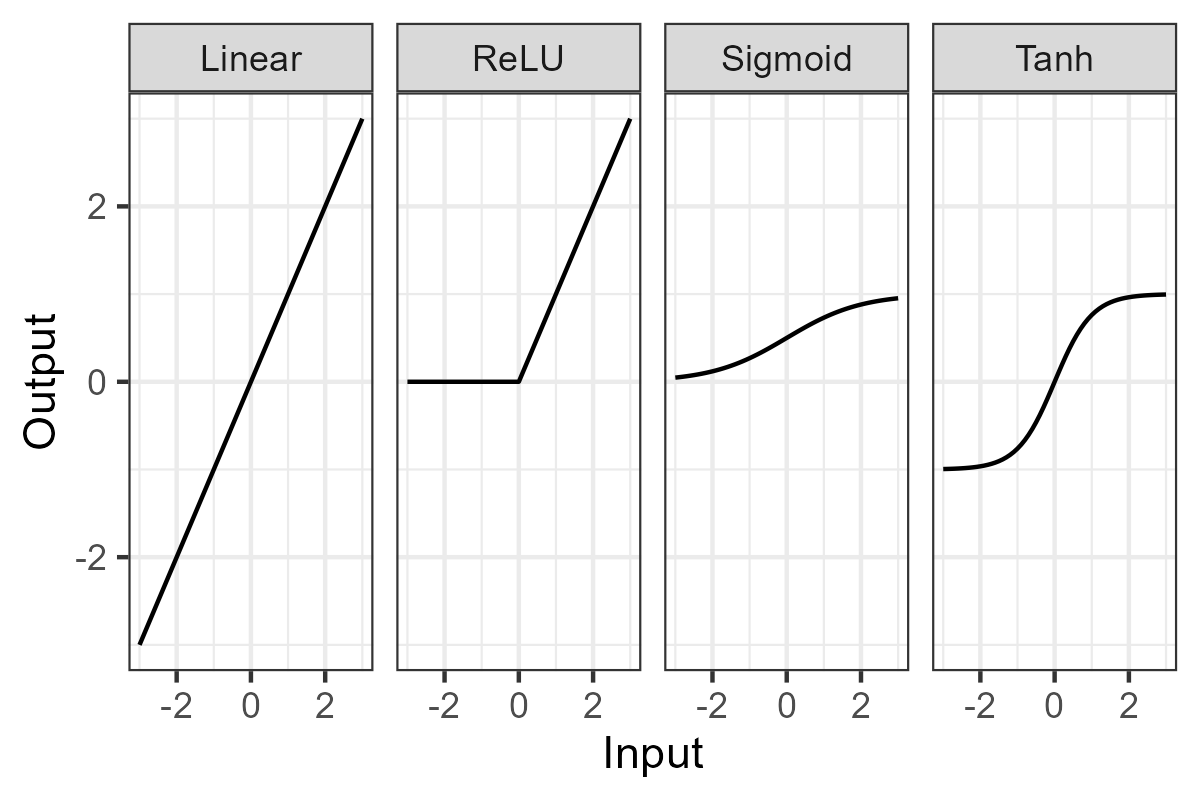
\includegraphics[width=0.8\linewidth]{"Figures/Activations.png"}
    \caption{A comparison of common activation functions. The purpose of this visualization is to show how the range of the inputs compares to the range of the outputs for different activations.}
    \label{fig:Activations}
\end{figure}

In addition to activation functions, each connection between nodes has a weight and bias. For example, the connection between $H_1$ and $X_1$ in Figure \ref{fig:NueralNetwork} would take the form:
\begin{equation*}
    H_1 = \sigma[w_1*X_1 + b_1]
\end{equation*}
where $\sigma[]$ indicates the activation function being applied, $w_1$ indicates the weight, and $b_1$ indicates the bias. The weights and biases in a network are what get tuned in the training process.

Training of neural networks occurs through the process of backpropogation, which is an application of the chain rule in calculus to determine how the output changes based on the change of a single parameter. The prediction of $y$ is compared to the observed value of $y$ in order to approximate a gradient, where each dimension represents a parameter. Then, gradient descent is used to find a minimum error, or loss, in the predictions.